\documentclass[tikz,border=10pt]{standalone}
\usepackage{tikz}

\begin{document}
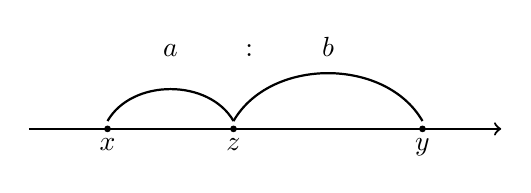
\begin{tikzpicture}

    \draw[thick,->] (0,0) -- (6,0);
    
    \filldraw[black] (1.0, 0) circle (1pt) node[below] {$x$};
    \filldraw[black] (2.6, 0) circle (1pt) node[below] {$z$};
    \filldraw[black] (5.0, 0) circle (1pt) node[below] {$y$};

    \draw[thick] (1,0.1) to[out=60,in=120] (2.6,0.1);
    \node[above] at (1.8,0.8) {$a$};

    \node[above] at (2.8,0.8) {$:$};
    
    \draw[thick] (2.6,0.1) to[out=60,in=120] (5,0.1);
    \node[above] at (3.8,0.8) {$b$};

\end{tikzpicture}
\end{document}